% main_formatted.tex
% E-Health for All: A User-Centered Telemedicine System
% IEEE Research Format with full Chapter 1 and Chapter 2 content

\documentclass[12pt]{report}

% -----------------------------------------------
% Packages
% -----------------------------------------------
\usepackage[margin=1in]{geometry}

\usepackage[T1]{fontenc}  % T1 encoding: full hyphenation patterns for long words
\usepackage{mathptmx}  % Times New Roman for pdfLaTeX
\usepackage[protrusion=true,expansion=true,nopatch=footnote]{microtype}  % Reduces overfull hboxes
\microtypesetup{stretch=30,shrink=20}  % Allow up to 3% font expansion

\usepackage{graphicx}
\graphicspath{{images/}}

\usepackage{booktabs}       % Professional table rules
\usepackage{array}          % Extended column options
\usepackage{amsmath}        % Math equations and formulas
\usepackage{amssymb}        % Math symbols
\usepackage{hyperref}       % Clickable citations and links
\hypersetup{
  colorlinks=true,
  linkcolor=black,
  citecolor=black,
  urlcolor=black
}
\usepackage{url}            % URL formatting
\usepackage{longtable}      % Tables spanning multiple pages
\usepackage{caption}        % Custom caption formatting
\usepackage{setspace}       % Line spacing control
\usepackage{enumitem}       % List formatting control
\usepackage{float}
\usepackage{indentfirst}
\usepackage{fancyhdr}

% -----------------------------------------------
% Page Style
% -----------------------------------------------
\pagestyle{fancy}
\fancyhf{}
\fancyfoot[R]{\thepage}
\renewcommand{\headrulewidth}{0pt}
\renewcommand{\footrulewidth}{0pt}
\setlength{\headheight}{15pt}
\addtolength{\topmargin}{-3pt}

% -----------------------------------------------
% Spacing
% -----------------------------------------------
\singlespacing
\setlength{\parindent}{0.5in}
\setlength{\parskip}{0pt}
\setlength{\emergencystretch}{3em}  % Fallback for lines microtype cannot fix
\hfuzz=2pt      % Suppress cosmetically invisible overfulls (< 0.7 mm)
\hbadness=10000 % Suppress underfull hbox warnings (common in bibliographies)

% -----------------------------------------------
% Chapter and Section Formatting
% -----------------------------------------------
\usepackage{titlesec}

% Chapter: centered, bold, 14pt, uppercase
\titleformat{\chapter}[block]
  {\normalfont\fontsize{14}{16}\bfseries\centering}
  {CHAPTER \thechapter:}{0.5em}{\MakeUppercase}
\titlespacing*{\chapter}{0pt}{0pt}{24pt}

% Section: bold, 12pt, left-aligned, title case
\titleformat{\section}
  {\normalfont\fontsize{12}{14}\bfseries}
  {\thesection}{1em}{}
\titlespacing*{\section}{0pt}{12pt}{6pt}

% Subsection: bold italic, 12pt
\titleformat{\subsection}
  {\normalfont\fontsize{12}{14}\bfseries\itshape}
  {\thesubsection}{1em}{}
\titlespacing*{\subsection}{0pt}{10pt}{4pt}

% -----------------------------------------------
% Caption Formatting
% -----------------------------------------------
\captionsetup{
  font={normalsize},
  labelfont={bf},
  labelsep=period,
  justification=centering,
  singlelinecheck=false
}

% -----------------------------------------------
% Bibliography
% -----------------------------------------------
\usepackage[backend=biber, style=ieee]{biblatex}
\addbibresource{references.bib}

% -----------------------------------------------
% Document Metadata
% -----------------------------------------------
\title{E-Health for All: A User-Centered Telemedicine System}
\author{Narvato, Dominnica SL.}

% -----------------------------------------------
% Begin Document
% -----------------------------------------------
\begin{document}

\fancypagestyle{plain}{%
  \fancyhf{}
  \fancyfoot[R]{\thepage}
  \renewcommand{\headrulewidth}{0pt}
}

%===============================================
% TITLE PAGE
%===============================================
\thispagestyle{empty}
\begin{center}
  \vspace*{1in}
  {\fontsize{14}{18}\bfseries E-Health for All: A User-Centered Telemedicine System\par}
  \vspace{1.5in}
  An Undergraduate Research Paper\\[6pt]
  Presented to the Faculty of the\\[6pt]
  College of Computer Studies\\[6pt]
  Naga College Foundation, Inc.\\[6pt]
  Naga City\\
  \vspace{1in}
  In Partial Fulfillment of\\[6pt]
  the Requirements for the Degree\\[6pt]
  Bachelor of Science in Information Systems\\
  \vspace{1in}
  Alinday, Mark Joseph M.\\[4pt]
  Bruzo, Ian\\[4pt]
  Narvato, Dominnica SL.\\[4pt]
  Paraiso, Kristine Carla I.\\[4pt]
  Villamer, EJ Andrei J.\\
  \vspace{1.5in}
  2027
\end{center}
\clearpage

%===============================================
% APPROVAL SHEET
%===============================================
\chapter*{\centering Approval Sheet}
\addcontentsline{toc}{chapter}{Approval Sheet}
\begin{center}
  {\bfseries NAGA COLLEGE FOUNDATION, INC.}\\[0.4em]
  {\bfseries COLLEGE OF COMPUTER STUDIES}\\[0.4em]
  {\bfseries NAGA CITY}\\[1.5em]
\end{center}

\noindent
This is to certify that the undergraduate research paper prepared by
\textbf{Alinday, Mark Joseph M., Bruzo, Ian, Narvato, Dominnica SL.,
Paraiso, Kristine Carla I., and Villamer, EJ Andrei J.}, entitled
\textbf{``E-Health for All: A User-Centered Telemedicine System''} submitted
in fulfillment of the requirements for the degree of Bachelor of Science in
Information Systems complies with the regulations of the institution and meets
the accepted standards with respect to originality.

\vspace{1.5em}
\noindent\textbf{Signed by the examination committee}
\vspace{1.5em}

\noindent
\begin{tabular}{p{4.5cm} p{3.5cm} p{3cm}}
  \toprule
  \textbf{Name} & \textbf{Signature} & \textbf{Date} \\
  \midrule
  \rule{4cm}{0.4pt} & \rule{3cm}{0.4pt} & \rule{2.5cm}{0.4pt} \\
  (Chairman) & & \\[1.5em]
  \rule{4cm}{0.4pt} & \rule{3cm}{0.4pt} & \rule{2.5cm}{0.4pt} \\
  (Panelist) & & \\[1.5em]
  \rule{4cm}{0.4pt} & \rule{3cm}{0.4pt} & \rule{2.5cm}{0.4pt} \\
  (Panelist) & & \\[1.5em]
  \rule{4cm}{0.4pt} & \rule{3cm}{0.4pt} & \rule{2.5cm}{0.4pt} \\
  (Adviser) & & \\[1.5em]
  \rule{4cm}{0.4pt} & \rule{3cm}{0.4pt} & \rule{2.5cm}{0.4pt} \\
  (Moderator) & & \\
  \bottomrule
\end{tabular}
\vfill
\clearpage

%===============================================
% CERTIFICATIONS & FRONT MATTER
%===============================================
\chapter*{\centering Secretary's Certification}
\addcontentsline{toc}{chapter}{Secretary's Certification}
\clearpage

\chapter*{\centering Editor's Certification}
\addcontentsline{toc}{chapter}{Editor's Certification}
\clearpage

\chapter*{\centering Statistician's Certification}
\addcontentsline{toc}{chapter}{Statistician's Certification}
\clearpage

\chapter*{\centering Acknowledgment}
\addcontentsline{toc}{chapter}{Acknowledgment}
\clearpage

\tableofcontents
\clearpage

\listoffigures
\clearpage

\listoftables
\clearpage

%===============================================
% ABSTRACT
%===============================================
\chapter*{\centering Abstract}
\addcontentsline{toc}{chapter}{Abstract}
% TODO: Add abstract here.
\clearpage

%===============================================
% CHAPTER 1: INTRODUCTION
%===============================================
\chapter{Introduction}

\indent In the Philippines, these challenges are especially severe. The
country's geography and urban concentration of medical specialists leave rural
populations with limited healthcare options. In response, the Philippine
government and health institutions have begun embracing telemedicine to broaden
coverage. The National Telehealth Center has launched SMS and web-based
platforms connecting rural patients with specialist consultations
\cite{ref25, ref59}, and various health institutions have adopted electronic
medical records to improve continuity of care across facilities
\cite{ref36, ref40}.

Despite these efforts, significant barriers persist. Poor transportation
infrastructure hinders facility access, particularly during emergencies and
follow-up care. Unreliable internet connectivity, limited computing resources,
and low digital literacy among both patients and healthcare workers further
compound these challenges \cite{ref1, ref46}. Existing telemedicine
initiatives, while promising, remain fragmented and rarely address the unique
technological constraints and cultural context of rural Filipino communities
\cite{ref49, ref51}.

This research seeks to bridge these gaps by developing an integrated
telemedicine platform specifically designed for the selected rural barangays.
The platform combines three components---a comprehensive doctors' database,
a patient records management system, and an appointment scheduling system---into
one user-friendly interface accessible to users with different levels of
digital literacy.

This initiative aligns with multiple UN Sustainable Development Goals: Good
Health and Well-Being (SDG 3), by improving healthcare access and quality;
Industry, Innovation, and Infrastructure (SDG 9), by demonstrating how
technology can address healthcare infrastructure gaps in underserved areas;
and Reduced Inequalities (SDG 10), by examining how digital health solutions
reduce disparities in healthcare access across different populations and
socioeconomic groups.

%-----------------------------------------------
\section*{Review of Related Literature}
%-----------------------------------------------

\subsection*{Telemedicine Adoption and Implementation}

Telemedicine, the delivery of healthcare services using information and
communication technologies, has emerged as a vital solution for healthcare
access issues in isolated and underserved communities. Telemedicine allows
healthcare providers to assess, diagnose, and treat patients in remote areas
by utilizing telecommunications technology to effectively connect medical
experts with populations that have limited access to healthcare facilities.
It has shown great promise in overcoming healthcare access issues in rural
communities around the world.

Research shows that telemedicine consultations promote better clinical
decision-making, reduce unnecessary patient transfers, and increase the chances
of local admissions instead of costly transfers to far-off hospitals
\cite{ref30, ref27}. These advantages apply to many medical fields, from
primary care to specialized areas like neurology and emergency medicine
\cite{ref15}.

However, the pandemic highlighted the shortcomings of telemedicine: access
services at lower rates \cite{ref10, ref21}. Digital literacy among older
adults and low-income individuals \cite{ref1, ref46}, equal access concerns
\cite{ref16, ref12, ref6}, implementation costs and maintenance \cite{ref43,
ref9}, infrastructure issues \cite{ref31, ref48, ref62}, and data security and
patient privacy concerns \cite{ref41}.

On the one hand, communities with integrated systems achieve better health
outcomes for managing chronic diseases compared to those that use fragmented
record-keeping \cite{ref32}. Patient satisfaction with telemedicine in the
Philippines shows encouraging trends \cite{ref32, ref39}. Even senior citizens
increasingly accepted remote consultations \cite{ref7}. The University of the
Philippines Health Service successfully used tailored electronic medical records
systems in various settings during COVID-19, ensuring continuity of patient
care despite mobility restrictions \cite{ref36, ref59}. Thorough assessments
show considerable progress in adoption over time, although significant gaps
between different types of facilities and locations persist \cite{ref3, ref38}.

Successfully implementing telemedicine requires careful adjustments to local
circumstances. Detailed analyses reveal Philippines-specific barriers like
governance issues, unclear licensure requirements, unresolved liability
problems, and vague reimbursement mechanisms that hinder healthcare provider
involvement \cite{ref25, ref51}. Healthcare technology must consider local
cultural practices, language preferences, and health-seeking behaviors to
ensure meaningful user acceptance in diverse Filipino communities \cite{ref49}.
Creating user-friendly systems is crucial for sustained adoption rather than
leaving behind abandoned pilot projects \cite{ref63}.

\subsection*{Patient Information Management System}

Patient information management involves the organized collection, storage, and
use of health data to support clinical decision-making and ensure continuity
of care. Electronic Medical Records (EMR) systems digitize patient health
information, enabling providers to access complete histories, track treatments,
identify medication interactions, and coordinate care across specialties. This
is especially critical in rural and underserved areas where access to prior
care records is limited.

EMR systems significantly improve care coordination, with integrated
communities achieving better chronic disease outcomes compared to those with
fragmented records \cite{ref33, ref19}. However, while basic adoption rates
are high, comprehensive implementation remains lower in rural facilities despite
recognized benefits \cite{ref12, ref6}. Technical, organizational, and workflow
barriers continue to hinder smooth information sharing \cite{ref48, ref3,
ref38}, and digital literacy gaps among older adults and low-income individuals
require targeted design and training interventions \cite{ref1}.

Data security and patient privacy are foundational to EMR trust, requiring
encryption, access controls, and audit trails \cite{ref41}. Integrated systems
reduce administrative burdens and improve care delivery \cite{ref45, ref56,
ref26}, while predictive models using patient data enable targeted interventions
and better resource allocation \cite{ref17, ref13}, supporting a shift toward
proactive, preventive primary care \cite{ref11}.

In the Philippines, EMR adoption shows both progress and challenges. COVID-19
visibly impacted system usage in rural health facilities \cite{ref2}, yet
implementation improved clinical decision-making and reduced medication errors
compared to paper systems \cite{ref40}. Sustained adoption is linked to
training, technical support, and gradual workflow integration rather than rapid
rollouts \cite{ref28}, though research representation across specialties,
settings, and facility types remains uneven \cite{ref14}. The absence of
centralized provider databases causes referral delays and disjointed care
\cite{ref60}, while comprehensive physician databases with specialization and
scheduling details enhance diagnostic workflows \cite{ref53}. Keeping such
databases accurate remains challenging, necessitating automated verification
and validation processes \cite{ref35}.

\subsection*{Appointment Scheduling in Healthcare}

Appointment scheduling systems are essential to healthcare delivery,
coordinating patient needs, provider availability, and facility resources.
Well-designed systems reduce waiting times, lower missed appointments through
automated reminders, improve provider productivity, and ensure urgent cases
receive prompt attention. In rural settings, where patients face long travel
distances and transportation barriers, efficient scheduling is especially
critical for maintaining access and treatment adherence.

Digital scheduling significantly reduces no-show rates compared to offline
booking, with automated reminders proving particularly effective \cite{ref45}.
AI-driven tools further improve efficiency by predicting non-attendance and
optimizing resource allocation \cite{ref56}, while open-access scheduling
reduces no-shows by offering same-day or next-day appointments \cite{ref26}.
Predictive models incorporating patient demographics and appointment history
identify high lead time and prior missed appointments as the strongest
predictors of non-attendance \cite{ref17, ref13}. Integrated systems also
improve patient flow and reduce waiting area congestion in underserved
facilities \cite{ref65}, supporting broader proactive primary care initiatives
through timely referrals and fewer missed appointments \cite{ref11, ref35}.

In the Philippines, digital appointment management in rural health centers has
shortened waiting times and reduced missed appointments through better time
slot management and automated reminders \cite{ref50}. However, rural contexts
require flexible approaches, as rigid scheduling is ineffective where patients
face unreliable transportation or inflexible work schedules. Systems must
therefore incorporate easy rescheduling options and reminder methods that
function without internet access \cite{ref37}.

%-----------------------------------------------
\section*{Synthesis of the State-of-the-Art}
%-----------------------------------------------

The detailed collection of works and studies offered valuable insights into the
topic. These studies backed their claims with relevant data and detailed
information.

Telemedicine has emerged as a viable solution to geographic barriers, improving
clinical decision-making, reducing unnecessary transfers, and expanding
specialist access \cite{ref15, ref30, ref27}. However, persistent challenges
remain, including infrastructure limitations, digital literacy gaps, data
security concerns, and Philippines-specific barriers such as unclear licensure,
liability, and reimbursement mechanisms \cite{ref25, ref41, ref46, ref51}.
Despite these, large-scale pilots in the Philippines demonstrate feasibility
across diverse communities, with patient satisfaction showing encouraging
trends even among senior citizens \cite{ref7, ref32, ref39, ref59}. Successful
adoption requires culturally sensitive, user-centered design tailored to local
contexts \cite{ref49, ref63}.

Patient information management systems significantly improve care coordination
and clinical outcomes, yet comprehensive EMR implementation remains lower in
rural facilities \cite{ref6, ref12}. Workflow barriers, digital literacy gaps,
and data security concerns continue to hinder full adoption
\cite{ref1, ref3, ref38, ref41}. In the Philippines, gradual integration
supported by training and technical assistance yields better sustained adoption
\cite{ref28}, while the absence of centralized provider databases causes
referral delays and fragmented care \cite{ref53, ref60}.

Appointment scheduling systems directly reduce no-show rates, improve patient
flow, and support proactive primary care \cite{ref11, ref45, ref56}. Predictive
modeling and AI-driven tools further optimize resource allocation
\cite{ref17, ref13, ref56}. In Philippine rural health centers, digital
scheduling has measurably shortened waiting times \cite{ref50}, though
flexible, offline-capable systems are essential given transportation and
connectivity constraints \cite{ref37}.

Across all three areas, the literature consistently points to the need for an
integrated, context-sensitive platform that unifies patient records, provider
information, and appointment scheduling---precisely the gap this research
addresses.

%-----------------------------------------------
\section*{Gap Bridged by the Study}
%-----------------------------------------------

This study addresses important gaps in rural healthcare delivery by creating an
integrated telemedicine platform specifically for rural barangays in Naga City.
Existing telemedicine systems often look at patient management and appointment
scheduling separately. This research offers a more complete solution by
combining a doctors' database, a patient records management system, and
appointment scheduling into one platform. It addresses the unreliable internet
connectivity that is common in rural areas. Healthcare workers can keep entering
data and accessing patient information even without internet access. Once the
connection is restored, the system syncs automatically. By bringing these
features together in one practical system designed for resource-limited
settings, this research shows how telemedicine solutions can be adapted to meet
the real technological, infrastructure, and cultural challenges faced in rural
healthcare.

%-----------------------------------------------
\section*{Theoretical Framework}
%-----------------------------------------------

This study is grounded in three key theories that collectively support the
development of the proposed telemedicine system: the Diffusion of Innovations
(DOI) Theory \cite{ref42}, the Task--Technology Fit (TTF) Theory \cite{ref52},
and the Technology Acceptance Model (TAM) \cite{ref58}. Together, these
theoretical foundations inform the system's design, usability considerations,
and adoption potential within rural healthcare settings.

According to Goodhue and Thompson (1995), the Task Technology Fit (TTF) Model
posits that technology will be adopted and effectively utilized when its
functionalities align with the specific tasks that users are expected to
perform. The model argues that a strong ``fit'' between task requirements---such
as information retrieval, decision-making, communication, and
documentation---and the capabilities of the system results in improved
individual performance and greater likelihood of continued system use. When
technology supports the user's workflow and reduces the effort required to
complete essential activities, it becomes more valuable, usable, and integrated
into daily operations. This model is relevant to the proposed telemedicine
platform because its success depends on how well its features---such as patient
record management, scheduling, and remote consultation support---match the
operational needs and constraints of rural healthcare providers \cite{ref52}.

According to Rogers (2020), the Diffusion of Innovations (DOI) Theory explains
how new ideas, practices, or technologies spread through a population over time.
It emphasizes understanding the characteristics of innovations and the social
processes that influence adoption rates among different groups \cite{ref42}.
The theory focuses on five key attributes that determine adoption: relative
advantage, compatibility, complexity, trialability, and observability. In this
study, it will guide the implementation strategy for the telemedicine platform
in rural communities. The strategy will consider social dynamics and adoption
patterns when introducing the system. The researcher can identify early
adopters, such as progressive healthcare providers and influential community
health workers, show its benefits to others, and help normalize its use in the
community.

According to Marikyan and Papagiannidis (2024), the Technology Acceptance
Model (TAM) asserts two significant factors in a user's intention to adopt a
technology: perceived usefulness and perceived ease of use \cite{ref58}.
Perceived usefulness refers to the extent to which an individual believes that
a technology enhances task performance and overall productivity, while perceived
ease of use pertains to the belief that the system can be operated with minimal
physical and cognitive effort. TAM is highly relevant to the proposed
telemedicine platform because its adoption depends on users---especially those
in rural areas with varying levels of digital literacy---perceiving the system
as beneficial, simple to navigate, and supportive of their essential healthcare
tasks.

\begin{figure}[!ht]
  \centering
  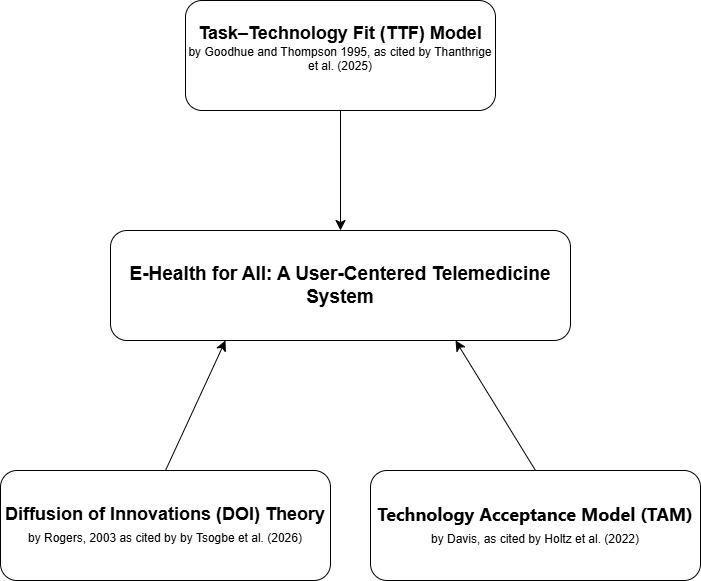
\includegraphics[width=0.85\textwidth]{Theoretical Paradigm.jpg}
  \caption{Theoretical Paradigm illustrating the DOI, TTF, and TAM frameworks
           guiding the E-Health for All telemedicine system development.}
  \label{fig:theoretical}
\end{figure}

%-----------------------------------------------
\section*{Conceptual Framework}
%-----------------------------------------------

The enhanced system paradigm is the approach utilized in the conceptualization
of this study. The input came from various sources to gain a complete
understanding of rural healthcare needs and readiness for technology, such as
document analysis of health records, observations of healthcare-seeking
behaviors and travel times, surveys evaluating user satisfaction and technology
skills, and interviews gathering in-depth information about access challenges
and provider readiness for telemedicine services.

The processes involved include: systems analysis and specification for system
design, functional testing to ensure adherence to system requirements, usability
testing to ensure the system meets user needs, and acceptability validation to
confirm system feasibility for deployment. The study's output is a web
application with features including computer vision, security, authentication,
verification, patient check-up history, and QR code security. The continuous
feedback mechanism will ensure iterative refinement of the system to remain
user-friendly, operational, and aligned with rural healthcare needs.

\begin{figure}[!h]
  \centering
  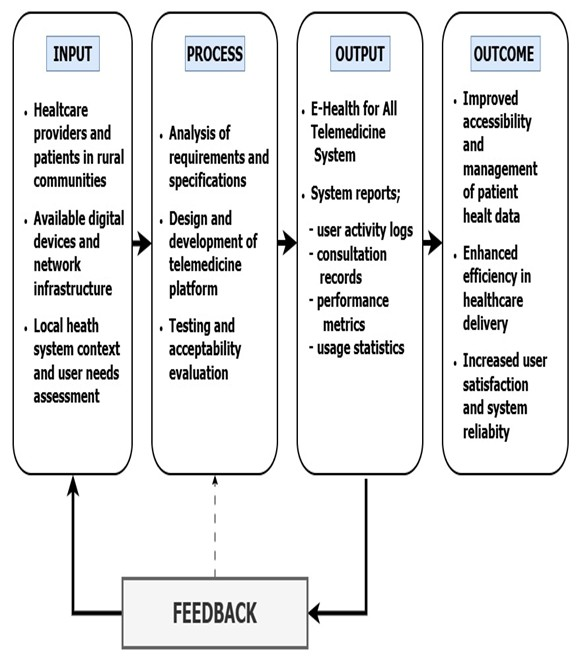
\includegraphics[width=0.90\textwidth]{Conceptual Paradigm.jpg}
  \caption{Conceptual Paradigm based on the Input-Process-Output-Outcome (IPOO)
           model illustrating the systematic development of the E-Health for All
           telemedicine system.}
  \label{fig:conceptual}
\end{figure}

%-----------------------------------------------
\section*{Statement of the Problem}
%-----------------------------------------------

This study aims to address the problem in healthcare accessibility of rural
populations. Specifically, this study seeks to answer the following questions:

\begin{enumerate}[label=\arabic*., leftmargin=0.75in, itemsep=4pt, parsep=0pt]
  \item What are the current practices of rural healthcare providers in rural
        populations with respect to:
        \begin{enumerate}[label=\alph*), leftmargin=0.5in, itemsep=2pt]
          \item Patient records management
          \item Doctor scheduling
          \item Appointment systems
        \end{enumerate}
  \item What are the challenges encountered in the current system with respect to:
        \begin{enumerate}[label=\alph*), leftmargin=0.5in, itemsep=2pt]
          \item Patient records management
          \item Doctor scheduling
          \item Appointment systems
        \end{enumerate}
  \item What system can be designed to address the challenges encountered?
  \item What is the level of acceptability of the system in terms of:
        \begin{enumerate}[label=\alph*), leftmargin=0.5in, itemsep=2pt]
          \item Usability
          \item Reliability
          \item Data security
        \end{enumerate}
\end{enumerate}

%-----------------------------------------------
\section*{Assumptions}
%-----------------------------------------------

The research study is anchored on the following key assumptions:

\begin{enumerate}[label=\arabic*., leftmargin=0.75in, itemsep=4pt, parsep=0pt]
  \item Rural healthcare providers in Panicuason, Naga City have specific
        practices for managing patient records, scheduling doctors, and handling
        appointments.
  \item There are challenges with the current systems for managing patient
        records, scheduling doctors, and setting up appointments in rural
        healthcare facilities.
  \item A user-centered telemedicine platform can be designed and developed to
        tackle these challenges in the current healthcare delivery system.
  \item The rural healthcare providers and clinic staff are ready to accept and
        shift from current manual practices toward the proposed user-friendly
        telemedicine platform and digital records management system.
\end{enumerate}

%-----------------------------------------------
\section*{Scope and Delimitation}
%-----------------------------------------------

This study addresses healthcare accessibility problems in rural populations,
specifically focusing on rural healthcare providers and their patients. The
objective of this study is to design a user-friendly online system to improve
the management of patient records, aid in scheduling providers, and assist in
arranging appointments to enable healthcare delivery to be more effective in
rural environments.

The study will be conducted in Barangay Panicuason, Naga City, covering the
entire design and development of a prototype for telemedicine functions,
including digital patient health profiles, clinical encounter documentation,
vital signs monitoring, medication monitoring, medical history access, and an
appointment scheduling system supported by an integrated doctor database. The
platform is a web application using a MySQL database and PHP, HTML, CSS, and
JavaScript with XAMPP local server for testing. It works on Windows 10/11,
macOS, Linux, and Android devices offline. The system only supports Android
smartphones running version 8.0 or higher with a minimum screen resolution of
$720 \times 1280$ pixels.

However, this study is limited only to Barangay Panicuason and does not extend
to other rural or urban healthcare facilities, which narrows the generalizability
of the findings. The system does not include high-level features such as lab
integration, payment and billing modules, pharmacy management, patient portals,
or iOS compatibility. Factors such as internet instability, power outages,
varying digital literacy levels, and changes in healthcare policies are also
beyond the study's scope.

%-----------------------------------------------
\section*{Significance of the Study}
%-----------------------------------------------

This research is important for various stakeholders and contributes to improving
healthcare equity and digital health innovation. The following are the key
beneficiaries:

\noindent\textbf{Patients in Rural Communities.} Rural residents will see the most direct
benefits by avoiding expensive trips to urban medical facilities for routine
check-ups. Patients save money on transportation and time spent traveling,
allowing them to access healthcare without disrupting work or family
responsibilities. Digital medical records give patients more health information,
while the appointment system cuts down on waiting times.

\noindent\textbf{Rural Healthcare Providers.} Healthcare providers in rural health units
will benefit from automated patient record management and better appointment
scheduling. Digital patient records allow for quicker clinical decisions,
especially during emergencies. The integrated doctors' database makes it easier
to refer patients to specialists and coordinate care.

\noindent\textbf{Community Health Workers.} Frontline workers gain better capabilities
through quick access to patient information for consultations and emergencies.
The system reduces paperwork, allowing them to focus on direct patient
interaction and health education. Workers can help facilitate remote
consultations for patients uncomfortable with technology and track health trends
to spot emerging issues early.

\noindent\textbf{Health Administrators and Local Government Officials.} Administrators
get valuable data on how telemedicine helps fill gaps in rural healthcare,
supporting better resource allocation decisions. The platform's reporting
features allow tracking of disease prevalence, service use, and community
healthcare needs.

\noindent\textbf{Technology Developers.} Technology developers get practical insights
into the technical needs and key features that are most important to rural
healthcare stakeholders. The research outlines detailed requirements for
building systems that can work offline and function well even with unreliable
internet access.

\noindent\textbf{Academic Researchers.} The research community benefits from clear
frameworks for creating easy-to-use digital health solutions for rural areas
with limited resources. This study offers evidence on effective design methods
and implementation techniques specifically made for resource-limited settings,
including validated tools for measuring how acceptable telemedicine is.

%-----------------------------------------------
\section*{Definition of Terms}
%-----------------------------------------------

\noindent\textbf{E-health.} E-health, also called electronic health or digital health,
refers to using information and communication technologies in healthcare
delivery \cite{ref66}. This includes telemedicine, electronic medical records,
and digital health platforms. It covers any health-related service or
information provided electronically through the internet, mobile devices, and
telecommunications systems to improve healthcare access, quality, and
efficiency.

\noindent\textbf{E-health for All.} The main principle and title of this research. It
highlights the need for equal access to digital health technologies for
everyone, regardless of where they live, their income, or their technology
skills \cite{ref20}. In this study, it means committing to creating inclusive,
user-friendly telemedicine solutions aimed specifically at rural communities in
Naga City.

\noindent\textbf{Telemedicine.} The delivery of healthcare services and clinical
information through communication technologies \cite{ref24}. This approach
helps overcome geographical barriers and improves access to medical services
for patients in remote areas.

\noindent\textbf{User-centered design.} A development methodology that focuses on the
needs, preferences, and limitations of end-users during the design process
\cite{ref55}. It involves actively engaging users in defining requirements,
evaluating prototypes, and refining systems.

\noindent\textbf{Rural healthcare.} Providing medical services in isolated or underserved
areas \cite{ref47}. These locations often lack adequate healthcare
infrastructure, have few medical specialists, and face significant barriers to
quality health services.

\noindent\textbf{Telehealth platform.} A digital health ecosystem that combines various
functions \cite{ref61}, including provider directories, patient information
systems, and scheduling tools to facilitate remote healthcare delivery and
improve care coordination.

\noindent\textbf{Healthcare accessibility.} How easily individuals can obtain necessary
health services on time. It considers factors like physical availability,
geographical proximity, economic affordability, and organizational fit.

\clearpage

%===============================================
% CHAPTER 2: METHODS
%===============================================
\chapter{Methods}

%-----------------------------------------------
\section*{Research Design}
%-----------------------------------------------

This study will adopt a developmental-descriptive qualitative research design.
This approach was chosen to describe and understand the current healthcare
access challenges in rural communities and to identify how telemedicine can
offer solutions. The descriptive method will help document the current state of
healthcare delivery and accessibility, and will provide detailed insights from
those who would use the telemedicine system daily.

Data will be collected through interviews, observations, and surveys, providing
understanding of how rural residents, healthcare providers, and community health
workers experience the current healthcare access situation. The study will also
include documentary analysis, where the researchers will review documents and
observe how healthcare services are accessed in these communities.

The study has four main phases: Phase 1 is the \textit{preparation phase},
where approvals are obtained and research tools are prepared. Phase 2 is the
\textit{assessment phase}, during which observation and documentation of the
current healthcare access situation are conducted. Phase 3 is the \textit{data
collection phase}, where the researchers conduct interviews and gather feedback.
Phase 4 is the \textit{analysis phase}, where all information is organized to
make recommendations.

\subsection*{Software Methodology}

The software development methodology for the E-Health for All application will
follow an iterative and incremental approach, combining elements of the Agile
methodology. Agile operates in short cycles where developers create small parts,
present them to users, gather feedback, and make improvements before proceeding.

\noindent\textbf{Development Phases.} The development will start with a list of all
necessary features based on research. Developers will create simple mockups and
share them with healthcare providers and rural residents. Programming will then
begin in phases:

\begin{enumerate}[label=\arabic*., leftmargin=0.75in, itemsep=2pt, parsep=0pt]
  \item User registration and doctor database
  \item Appointment scheduling
  \item Video consultations and patient records
  \item Prescription management
\end{enumerate}

\noindent\textbf{Testing Process.} Testing will occur before launch. Developers will
test the platform on different devices and internet speeds. Healthcare providers
will conduct mock consultations, while rural residents will test the mobile app.
Security testing will ensure that patient data is protected.

\noindent\textbf{Pilot Implementation.} Pilot testing in selected barangays will
identify issues before the full rollout. Training will be provided to healthcare
providers, community health workers, and rural residents.

%-----------------------------------------------
\section*{System Design}
%-----------------------------------------------

The system design process employed several modeling techniques such as use case
and system workflows to map user interactions and operational processes. These
techniques directly captured the functional requirements, user actions, and
step-by-step procedures within the system.

\subsection*{Use Case}

The use case diagram shows the specific interactions between patients, healthcare
providers, and system administrators with the system. In the use case diagram,
there were three actors: patients, doctors, and system administrators. All
actors can register and log in to the system. Patients and doctors utilize a
mobile application, while system administrators access a dedicated website
application.

\begin{figure}[H]
  \centering
  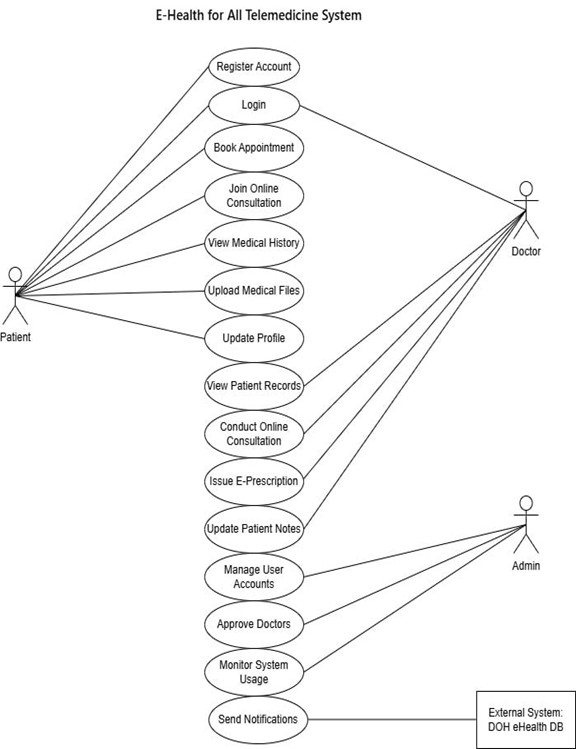
\includegraphics[width=0.90\textwidth]{Use Case Diagram.jpg}
  \caption{Use Case Diagram of the E-Health for All Telemedicine System.}
  \label{fig:usecase}
\end{figure}

\subsection*{System Workflows}

The system workflows illustrate the sequential processes and decision points
for key operations within the E-Health for All Telemedicine System. These
workflows ensure standardized procedures and guide users through various system
functionalities.

\begin{figure}[H]
  \centering
  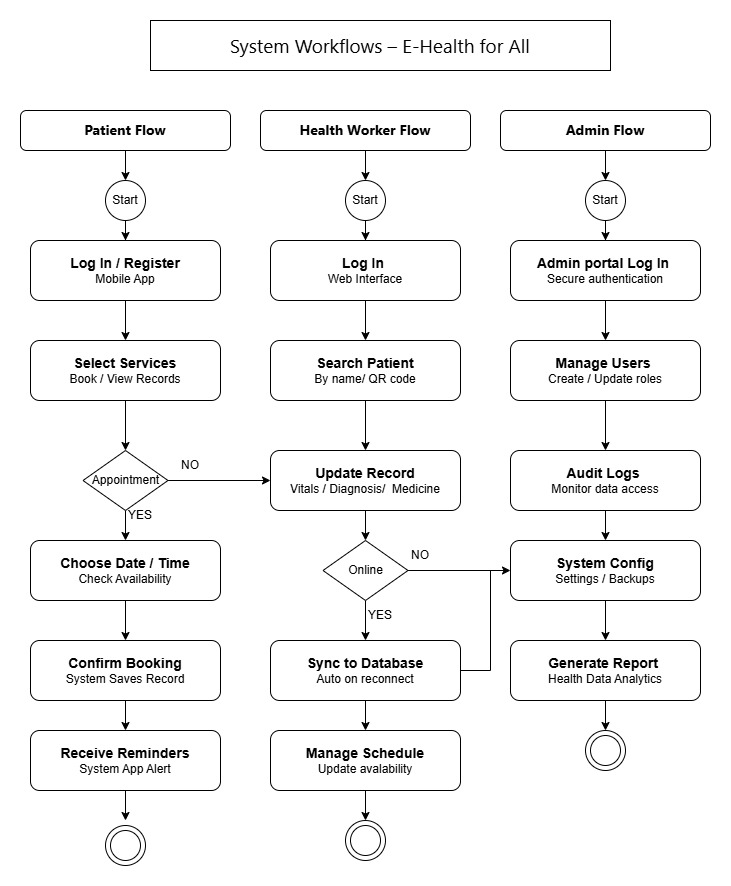
\includegraphics[width=0.90\textwidth]{System Workflows.jpg}
  \caption{System Workflows of the E-Health for All Telemedicine System.}
  \label{fig:workflows}
\end{figure}

\subsection*{Systems Architecture}

The system architecture for the E-Health for All Telemedicine System integrates
three key stakeholders: Healthcare Providers (Doctors), Rural residents, and
System Administrators. The proposed system comprises three main components
reflected in the Application Layer of the architecture:

\begin{enumerate}[label=\arabic*., leftmargin=0.75in, itemsep=4pt, parsep=0pt]
  \item \textbf{Web-based platform for healthcare providers}---includes
        secure login, patient record management, video consultation features,
        and the ability to document symptoms, diagnoses, and prescriptions.
  \item \textbf{Mobile application for rural residents}---allows users to
        schedule appointments, access medical records, conduct video
        consultations, receive appointment reminders via SMS, and access health
        education information.
  \item \textbf{Doctor database and scheduling system}---maintains provider
        profiles including specializations, qualifications, availability, and
        consultation fees.
\end{enumerate}

\begin{figure}[H]
  \centering
  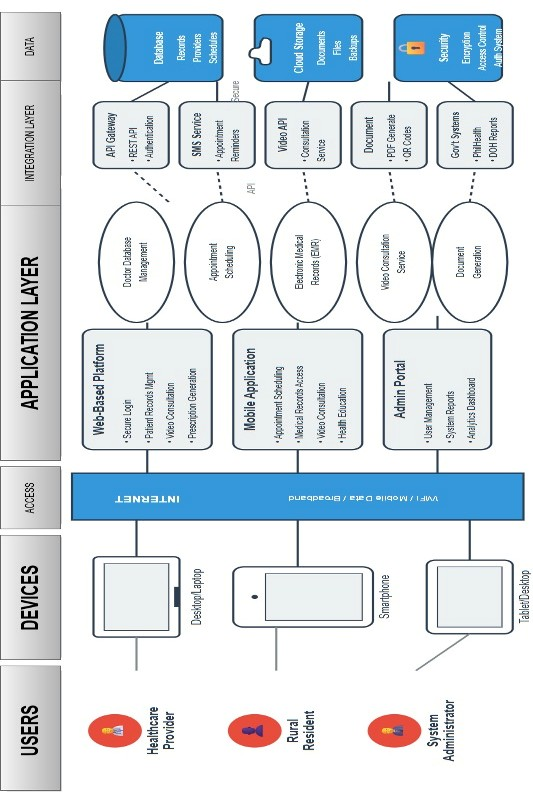
\includegraphics[width=0.85\textwidth]{E-Health for All System design Architecture.jpg}
  \caption{System Architecture of the E-Health for All Telemedicine System.}
  \label{fig:architecture}
\end{figure}

%-----------------------------------------------
\section*{Population and Sample}
%-----------------------------------------------

The researcher determined the respondents through a systematic selection process
based on their direct involvement with rural healthcare delivery at Panicuason
Barangay Health Center in Naga City. The study involved healthcare providers
and staff from Panicuason Rural Health Unit in Naga City.

Based on preliminary observation, the barangay health center has a total of 11
healthcare personnel consisting of 7 Dental Health Workers (DHW), 1 Midwife,
1 Encoder, 1 Barangay Nutrition Scholar (BNS), and 1 Staff Nurse (SNF). Since
there are only 11 respondents, the study will utilize total enumeration as the
sampling procedure for the design of the system.

For the rural community residents, purposive sampling will be implemented.
The sample size for rural residents is determined using Slovin's formula:

\begin{equation}
  n = \frac{N}{1 + N e^{2}}
  \label{eq:slovin}
\end{equation}

\noindent where:
\begin{itemize}[leftmargin=1in, itemsep=2pt, parsep=0pt]
  \item $n$ = required sample size
  \item $N$ = total population of Barangay Panicuason
  \item $e$ = margin of error (set at $0.05$ or $5\%$)
\end{itemize}

\noindent This formula helps ensure our sample size is adequate to represent the barangay
population while maintaining statistical reliability.

%-----------------------------------------------
\section*{Research Locale}
%-----------------------------------------------

The study will be conducted at Barangay Panicuason Rural Health Unit in Naga
City, Camarines Sur. Barangay Panicuason is located outside the urban center
of Naga City and faces typical rural healthcare challenges including limited
specialist availability and equipment, long travel distances to medical
facilities, and insufficient healthcare infrastructure.

The Rural Health Unit serves as the primary healthcare facility for residents
of Barangay Panicuason and surrounding areas. The facility provides basic health
services including primary care consultations, maternal and child health
programs, immunization services, disease prevention activities, and health
education.

%-----------------------------------------------
\section*{Data Gathering Procedure}
%-----------------------------------------------

\noindent\textbf{Preparation Phase.} This is the first step in establishing formal
agreements and obtaining necessary approvals before starting the research. It
involves getting approval and preparing formal letters to request permission
from barangay officials and local health officers, and creating consent forms
for all participants.

\noindent\textbf{Document Analysis.} This method collects data by examining health
records from barangay health stations, existing referral systems, and community
health profiles. The researchers will analyze: types of health complaints
commonly addressed, frequency of referrals to distant facilities, travel time
and costs to access healthcare, availability of medical specialists, and
community health statistics.

\noindent\textbf{Direct Observation.} This method involves systematically watching and
recording healthcare access patterns and challenges in their natural setting.
The researchers will take detailed notes about healthcare-seeking behavior,
time travel to the nearest clinic or hospital, document available transportation
options, and observe how health workers currently handle patient consultations
and referrals.

\noindent\textbf{Surveys.} This method collects information from respondents through
standardized questions and response options. It gives respondents a chance to
share their views, preferences, and experiences about current healthcare access
and their needs for a telemedicine solution.

\noindent\textbf{Interviews.} This method gathers information through one-on-one
conversations with stakeholders, allowing for deeper exploration of issues and
concerns. The researchers will conduct individual interviews lasting 30 to 45
minutes with rural residents, healthcare providers, and IT personnel.

%-----------------------------------------------
\section*{Validation and Testing Methods}
%-----------------------------------------------

\noindent\textbf{Functionality Testing.} Unit testing verified individual components,
with each function tested independently to ensure correct performance. Test
cases covered normal inputs, edge cases, and invalid inputs. Integration testing
verified module interactions, ensuring data flowed correctly between modules.

\noindent\textbf{User Acceptance Testing.} Healthcare providers evaluated whether the
system met their needs. Sign-off criteria required at least 80 percent feature
acceptance. Features falling below this threshold were revised based on
feedback.

\noindent\textbf{Performance Testing.} Load testing simulated multiple concurrent users,
testing the system with 10, 20, and 30 simultaneous users to ensure acceptable
performance under typical and peak loads. Target response times were set under
3 seconds for most operations.

\noindent\textbf{Security Testing.} Access control verification ensured users could only
access features appropriate to their roles. Data encryption validation confirmed
sensitive information was encrypted in transit using HTTPS and at rest in the
database.

\noindent\textbf{Usability Testing.} The think-aloud protocol was employed with 5 to 8
representative users. Task completion rates measured how many users successfully
completed tasks. Time-on-task measured efficiency. Error rates counted mistakes
made during tasks.

%-----------------------------------------------
\section*{Research Instrument}
%-----------------------------------------------

\noindent\textbf{Interview Guides.} Researchers will prepare interview guides for rural
residents of Barangay Panicuason covering: experiences with healthcare services
at the barangay health center, distance traveled to see a doctor, costs involved
in getting medical care, health problems commonly faced, access to mobile phones
and the internet, comfort level with technology, and desired features in a
telemedicine platform.

\noindent\textbf{Survey Questionnaires.} For rural residents, the questionnaire will ask
about their age, household size, and common health conditions. Other questions
will include: satisfaction with current healthcare access using a 5-point scale,
distance traveled to see a doctor, healthcare spending, frequency of delaying
medical care, mobile phone and internet access, and preferred telemedicine
features.

%-----------------------------------------------
\section*{Ethical Considerations}
%-----------------------------------------------

\noindent\textbf{Voluntary Participation.} Participation in this study is completely
voluntary. No one will be pressured or given incentives that could unduly
influence their decision to join. Participants can withdraw at any time without
consequences.

\noindent\textbf{Informed Consent.} All participants received detailed information about
the study before agreeing to participate. This information covered the study's
purpose, what participation involved, how data would be collected and used,
potential risks and benefits, confidentiality measures, and the right to
withdraw.

\noindent\textbf{Parental/Guardian Consent and Minor Assent.} For participants under 18
years of age, written parental or legal guardian consent will be obtained before
any research involvement. Minors aged 7--17 years will also provide written
assent. Minors may decline participation even if parents have provided consent.

\noindent\textbf{Privacy and Confidentiality.} Individual identities will not be
revealed without explicit written permission. Interview recordings and
transcripts will be stored in password-protected digital files accessible only
to the research team.

\noindent\textbf{Data Protection.} All research data will be handled according to the
Data Privacy Act of 2012 (Republic Act No. 10173). Personal identifiers will
be removed from datasets, and survey responses will remain anonymous.

%-----------------------------------------------
\section*{Statistical Tools}
%-----------------------------------------------

\subsection*{Descriptive Statistics}

The study employed descriptive statistical methods to summarize and describe
the characteristics of the sample and their responses.

\noindent\textbf{Percentage.} To show the proportion of respondents who chose each
answer option, percentages are calculated using the formula:

\begin{equation}
  P = \frac{f}{N} \times 100
  \label{eq:percentage}
\end{equation}

\noindent where $f$ is the frequency or number of responses for a specific
option and $N$ is the total number of respondents.

\noindent\textbf{Weighted Mean.} For Likert-scale items, the weighted mean is calculated
using the formula:

\begin{equation}
  \bar{x} = \frac{\sum (W \cdot f)}{N}
  \label{eq:weightedmean}
\end{equation}

\noindent where $W$ is the weight or scale value (1--5 for a 5-point Likert
scale), $f$ is the frequency of respondents who chose that value, and $N$ is
the total number of respondents.

\subsection*{Frequency Distribution}

Frequency tables display how many respondents selected each response option.
Table~\ref{tab:frequency} shows a sample frequency distribution for a
5-point satisfaction scale.

\begin{table}[htbp]
  \centering
  \caption{Sample Frequency Distribution of Respondent Satisfaction}
  \label{tab:frequency}
  \begin{tabular}{lcc}
    \toprule
    \textbf{Response Category} & \textbf{No. of Respondents} &
    \textbf{Percentage} \\
    \midrule
    Very Satisfied    & 5  & 8.3\%   \\
    Satisfied         & 25 & 41.7\%  \\
    Neutral           & 15 & 25.0\%  \\
    Dissatisfied      & 10 & 16.7\%  \\
    Very Dissatisfied & 5  & 8.3\%   \\
    \midrule
    \textbf{Total}    & \textbf{60} & \textbf{100\%} \\
    \bottomrule
  \end{tabular}
\end{table}

\subsection*{Statistical Treatment of Data}

The data gathered will be interpreted using a five-point Likert scale to measure
the respondents' attitudes, opinions, perceptions, and preferences regarding the
user-centered telemedicine system. Table~\ref{tab:likert} shows the
interpretation scale used for weighted mean values.

\begin{table}[htbp]
  \centering
  \caption{Likert Scale for Agreement on Telemedicine System Acceptability}
  \label{tab:likert}
  \begin{tabular}{ccc}
    \toprule
    \textbf{Scale} & \textbf{Range} & \textbf{Interpretation} \\
    \midrule
    5 & 4.21 -- 5.00 & Strongly Agree   \\
    4 & 3.41 -- 4.20 & Agree            \\
    3 & 2.61 -- 3.40 & Neutral          \\
    2 & 1.81 -- 2.60 & Disagree         \\
    1 & 1.00 -- 1.80 & Strongly Disagree \\
    \bottomrule
  \end{tabular}
\end{table}

%-----------------------------------------------
\section*{Project Timeline}
%-----------------------------------------------

Table~\ref{tab:timeline} outlines the systematic schedule of activities for
conducting the research study on the user-centered telemedicine system.

\begin{table}[htbp]
  \centering
  \caption{Project Timeline from Preparation Phase to Prototype Implementation}
  \label{tab:timeline}
  \small
  \begin{tabular}{lcccccccc}
    \toprule
    \textbf{Activity} & \textbf{M1} & \textbf{M2} & \textbf{M3} &
    \textbf{M4} & \textbf{M5} & \textbf{M6} & \textbf{M7} & \textbf{M8} \\
    \midrule
    \multicolumn{9}{l}{\textit{Preparation Phase}} \\
    Finalize proposal and instruments
      & $\bullet$ & $\bullet$ & & & & & & \\
    Obtain approvals and permissions
      & $\bullet$ & $\bullet$ & & & & & & \\
    Pilot test instruments
      & $\circ$   & $\circ$   & & & & & & \\
    \midrule
    \multicolumn{9}{l}{\textit{Data Collection -- Observations}} \\
    Observation in Panicuason
      & & $\bullet$ & $\bullet$ & & & & & \\
    Document analysis
      & & $\bullet$ & $\bullet$ & & & & & \\
    \midrule
    \multicolumn{9}{l}{\textit{Data Collection -- Stakeholder Input}} \\
    Individual interviews
      & & & $\bullet$ & $\bullet$ & & & & \\
    Survey distribution and collection
      & & & $\bullet$ & $\bullet$ & & & & \\
    \midrule
    \multicolumn{9}{l}{\textit{Data Analysis}} \\
    Transcription
      & & & & & $\bullet$ & $\bullet$ & & \\
    Coding and thematic analysis
      & & & & & $\circ$   & $\bullet$ & & \\
    Statistical analysis
      & & & & & & $\circ$   & & \\
    \midrule
    \multicolumn{9}{l}{\textit{Report Writing}} \\
    Findings documentation
      & & & & & & $\circ$ & $\circ$ & $\bullet$ \\
    Final report preparation
      & & & & & & & $\bullet$ & $\bullet$ \\
    \bottomrule
    \multicolumn{9}{l}{Legend: $\bullet$ = Active work period;\quad
                                $\circ$ = Overlap or transitional period} \\
  \end{tabular}
\end{table}

\clearpage

%===============================================
% CHAPTER 3: RESULTS AND DISCUSSIONS
%===============================================
\chapter{Results and Discussions}

%-----------------------------------------------
\section*{Results}
%-----------------------------------------------

\subsection*{Problem 1: Current Practices of Rural Healthcare Providers}
% TODO: Add findings here

\subsection*{Problem 2: Challenges in the Current System}
% TODO: Add findings here

\subsection*{Problem 3: System Design to Address Challenges}
% TODO: Add findings here

%-----------------------------------------------
\section*{Design and System Plans}
%-----------------------------------------------
% TODO

%-----------------------------------------------
\section*{Summary of Findings}
%-----------------------------------------------
% TODO

%-----------------------------------------------
\section*{Conclusions}
%-----------------------------------------------
% TODO

%-----------------------------------------------
\section*{Recommendations}
%-----------------------------------------------
% TODO

%===============================================
% REFERENCES
%===============================================
\clearpage
\printbibliography

\clearpage
\chapter*{Curriculum Vitae}
\addcontentsline{toc}{chapter}{Curriculum Vitae}

\clearpage
\chapter*{Appendices}
\addcontentsline{toc}{chapter}{Appendices}

\end{document}
